\chapter{Chromatography}\label{ch:b2:chromatography}

A drop of an energy drink, diluted and filtered, is injected into a steel tube no longer than a pen and
packed with silica grains a few micrometres across. A few minutes later a detector has drawn a line
with a handful of peaks, and from the area of one of them the laboratory reports how much caffeine the
can holds, to a few per cent. \omterm{def:b2:chromatography:principle}{Chromatography} separates the components of a mixture by letting them
race through a column at different speeds; this chapter explains why they travel at different speeds,
why their peaks have the width they have, how to separate two neighbours, and how to turn a peak into
a quantity.

\begin{omfigure}
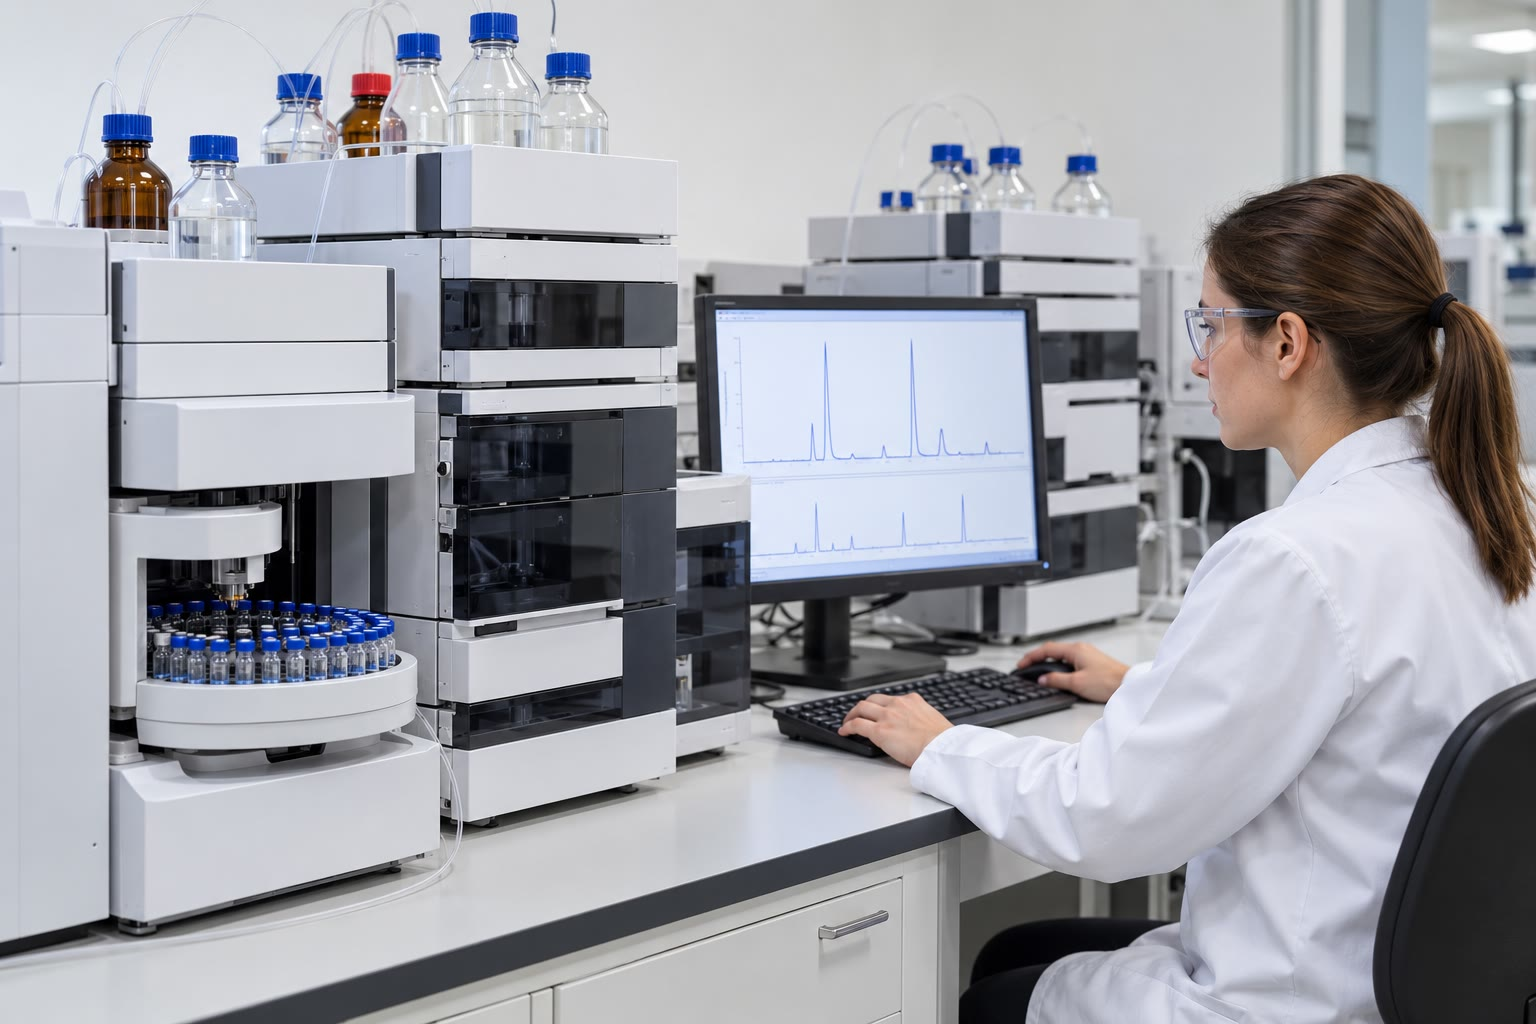
\includegraphics[width=0.58\linewidth]{images/book3/ai/b2-31-analytical-lab.jpg}

{\small An analytical laboratory: liquid chromatographs with their solvent bottles and an autosampler
tray of vials; the chromatograms appear on the screen (illustration).}
\end{omfigure}

\begin{recall}
The school volume: paper and thin-layer \omterm{def:b2:chromatography:principle}{chromatography}, chromatogram, eluent. The Year 1 volume: the
partition coefficient, liquid--liquid extraction, the retention factor $R_f$ of a thin-layer plate.
\Cref{ch:b2:liquid-vapour-diagrams}: the \omterm{def:b2:liquid-vapour-diagrams:fractional-distillation}{theoretical plate} of a distillation column.
\end{recall}

\section{Principle}

\begin{definition}[Chromatography]\label{def:b2:chromatography:principle}
\emph{Chromatography}\index{chromatography} separates the components of a mixture by distributing them
between a \emph{stationary phase}\index{stationary phase}, fixed in a column or on a plate, and a
\emph{mobile phase}\index{mobile phase}, a gas or a liquid that flows past it. Carrying the components
through and out of the column with the mobile phase is \emph{elution}\index{elution}.
\end{definition}

A molecule moves only while it is in the \omterm{def:b2:chromatography:principle}{mobile phase}; while it is held by the \omterm{def:b2:chromatography:principle}{stationary phase} it
waits. It switches between the two phases millions of times on its way, so its average speed is set by
the fraction of time it spends in each, that is by its partition equilibrium.

\begin{definition}[Retention]\label{def:b2:chromatography:retention}
The \emph{retention time}\index{retention time} $t_R$ of a compound is the time from injection to the
maximum of its peak; the \emph{hold-up time}\index{hold-up time} $t_M$ is the retention time of an
unretained compound, which never enters the \omterm{def:b2:chromatography:principle}{stationary phase}. The \emph{retention factor}\index{retention factor k@retention factor $k$}
$k$ of a compound on a column is
\begin{equation*}
k = \frac{t_R - t_M}{t_M}.
\end{equation*}
It is not the $R_f$ of a thin-layer plate, which measures a distance travelled, though both describe
the same partition.
\end{definition}

\begin{proposition}[Retention time]\label{prop:b2:chromatography:retention-time}
If, at equilibrium, the amounts of a compound in the stationary and \omterm{def:b2:chromatography:principle}{mobile phases} of a slice of column
are $n_s$ and $n_m$, the compound moves at $u/(1 + n_s/n_m)$, where $u$ is the speed of the \omterm{def:b2:chromatography:principle}{mobile phase},
and $t_R = t_M(1 + n_s/n_m)$.
\end{proposition}

\begin{proof}
A given molecule spends the fraction $n_m/(n_s + n_m)$ of its time in the \omterm{def:b2:chromatography:principle}{mobile phase}, where it moves at
$u$, and the rest at rest. Its average speed is $u\,n_m/(n_s + n_m) = u/(1 + n_s/n_m)$. The column of
length $L$ is crossed in $t_R = (L/u)(1 + n_s/n_m)$, and $L/u = t_M$.
\end{proof}

\begin{proposition}[Retention and partition]\label{prop:b2:chromatography:k-and-K}
The \omterm{def:b2:chromatography:retention}{retention factor} is the ratio of the amounts in the two phases, $k = n_s/n_m = KV_s/V_m$, where $K$
is the partition coefficient (concentration in the \omterm{def:b2:chromatography:principle}{stationary phase} over concentration in the \omterm{def:b2:chromatography:principle}{mobile
phase}) and $V_s$, $V_m$ the volumes of the phases in the column.
\end{proposition}

\begin{proof}
From \cref{prop:b2:chromatography:retention-time}, $(t_R - t_M)/t_M = n_s/n_m$. With $n_s = c_sV_s$,
$n_m = c_mV_m$ and $K = c_s/c_m$, $n_s/n_m = KV_s/V_m$.
\end{proof}

Two compounds separate if their partition coefficients differ; the column geometry ($V_s/V_m$)
multiplies all retentions alike. Changing the \omterm{def:b2:chromatography:principle}{mobile phase}, which changes $K$, is the chemist's main
lever on retention.

\begin{omfigure}
\begin{tikzpicture}[x=1cm, y=1cm]
\foreach \x/\a/\b/\ha/\hb/\lab in {0/0.6/0.6/0.1/0.1/start, 2.4/1.5/2.6/0.16/0.22/later, 4.8/2.4/4.4/0.2/0.3/end}{
  \draw[black!60] (\x-0.35,0) rectangle (\x+0.35,-5);
  \fill[omThm!55] (\x-0.33,-\b+\hb) rectangle (\x+0.33,-\b-\hb);
  \fill[omDef!55, opacity=0.85] (\x-0.33,-\a+\ha) rectangle (\x+0.33,-\a-\ha);
  \node[font=\small] at (\x,-5.4) {\lab};
}
\draw[->, thick] (-1.0,-0.3) -- (-1.0,-4.6) node[midway, left, font=\small, align=right] {mobile\\phase};
\node[font=\small, align=left, anchor=west] at (5.5,-2.4) {more retained\\(slow, narrow)};
\node[font=\small, align=left, anchor=west] at (5.5,-4.4) {less retained\\(fast)};
\draw[densely dotted] (5.15,-2.4) -- (5.5,-2.4); \draw[densely dotted] (5.15,-4.4) -- (5.5,-4.4);
\end{tikzpicture}
\par\vspace{4pt}

{\small Two compounds injected together as one thin band move down a column (three snapshots,
schematic). The less retained one (smaller $k$) runs ahead; both bands widen as they travel, the one
that has gone further the more.}
\end{omfigure}

\section{Peak width and plate number}

A band does not stay thin. Molecules of the same compound take different paths between the grains,
diffuse along the column and lag behind in the \omterm{def:b2:chromatography:principle}{stationary phase} by random amounts. The peak recorded at
the outlet is very nearly a Gaussian of standard deviation $\sigma_t$ (in time), and the narrower it is
for a given $t_R$, the better the column.

\begin{definition}[Plate number]\label{def:b2:chromatography:plates}
The \emph{plate number}\index{plate number} of a column for a compound is $N = (t_R/\sigma_t)^2$, where
$\sigma_t$ is the standard deviation of its peak in time. The \emph{plate height}\index{plate height} is
$H = L/N$, for a column of length $L$.
\end{definition}

The names come from the distillation column of \cref{ch:b2:liquid-vapour-diagrams}: a chromatographic
column behaves as if it were a stack of $N$ equilibrium stages, each $H$ high. The analogy is a way of
counting, not a picture of the column.

\begin{proposition}[Plate number from a peak]\label{prop:b2:chromatography:plate-number}
With $w$ the width at the base between the tangents at the inflection points and $w_{1/2}$ the width at
half height,
\begin{equation*}
N = 16\left(\frac{t_R}{w}\right)^2 = 5.54\left(\frac{t_R}{w_{1/2}}\right)^2.
\end{equation*}
\end{proposition}

\begin{proof}
For a Gaussian of standard deviation $\sigma$ and height $h$, the inflection points are at $\pm\sigma$,
where the height is $h\mathrm e^{-1/2}$ and the slope $\mp h\mathrm e^{-1/2}/\sigma$; the tangent there
reaches zero after $\sigma$ more, at $\pm2\sigma$: $w = 4\sigma$. Half height is reached where
$\mathrm e^{-x^2/2\sigma^2} = 1/2$, $x = \sigma\sqrt{2\ln2}$: $w_{1/2} = 2\sqrt{2\ln2}\,\sigma \approx
2.355\,\sigma$. Substituting $\sigma = w/4$ or $\sigma = w_{1/2}/2.355$ in $N = (t_R/\sigma)^2$ gives
$16$ and $2.355^2 = 5.545$, written 5.54.
\end{proof}

\begin{proposition}[Van Deemter equation]\label{prop:b2:chromatography:van-deemter}
The \omterm{def:b2:chromatography:plates}{plate height} depends on the linear speed $u$ of the \omterm{def:b2:chromatography:principle}{mobile phase} as
\begin{equation*}
H = A + \frac{B}{u} + Cu,
\end{equation*}
where $A$ accounts for the different paths through the packing, $B/u$ for diffusion along the column
(worse when the molecules stay longer) and $Cu$ for the slow exchange with the \omterm{def:b2:chromatography:principle}{stationary phase} (worse
when the \omterm{def:b2:chromatography:principle}{mobile phase} hurries past). $H$ is smallest at $u_{\mathrm{opt}} = \sqrt{B/C}$, where $H_{\min} =
A + 2\sqrt{BC}$.
\end{proposition}

\admitted

The form of the equation is admitted; its minimum is not. $\mathrm dH/\mathrm du = -B/u^2 + C$ vanishes
at $u = \sqrt{B/C}$, and there $B/u = Cu = \sqrt{BC}$, so $H_{\min} = A + 2\sqrt{BC}$; the second
derivative $2B/u^3$ is positive, so this is a minimum. Small grains reduce $A$ and $C$: that is why
modern liquid \omterm{def:b2:chromatography:principle}{chromatography} uses particles of a few micrometres and high pressures to push the \omterm{def:b2:chromatography:principle}{mobile
phase} through them.

\begin{omfigure}
\begin{tikzpicture}
\begin{axis}[width=0.7\linewidth, height=5.2cm, xmin=0, xmax=8, ymin=0, ymax=70,
  xlabel={linear speed $u$ (\unit{mm/s})}, ylabel={plate height $H$ (\unit{\micro m})},
  label style={font=\small}, tick label style={font=\scriptsize},
  legend style={font=\scriptsize, at={(1.03,1)}, anchor=north west}, legend cell align=left]
\addplot[omDef, very thick] table[x=u, y=H] {figdata/out/bachelor-2-chromatogram-b.dat};
\addplot[black!50, dashed] table[x=u, y=A] {figdata/out/bachelor-2-chromatogram-b.dat};
\addplot[omThm, dashed] table[x=u, y=B] {figdata/out/bachelor-2-chromatogram-b.dat};
\addplot[omMeth, dashed] table[x=u, y=C] {figdata/out/bachelor-2-chromatogram-b.dat};
\addplot[only marks, mark=*, mark size=1.6pt] coordinates {(2,30)};
\legend{$H$, $A$, $B/u$, $Cu$}
\end{axis}
\end{tikzpicture}

{\small A van Deemter curve (exercise parameters: $A = \qty{10}{\micro m}$, $B = \qty{20}{\micro m.mm/s}$,
$C = \qty{5}{\micro m.s/mm}$). The minimum, $H = \qty{30}{\micro m}$ at $u = \qty{2}{mm/s}$, sits where
the diffusion and exchange terms are equal.}
% figdata: bachelor-2/chromatogram.py part b
\end{omfigure}

\section{Separating two compounds}

\begin{definition}[Selectivity and resolution]\label{def:b2:chromatography:separation}
For two neighbouring peaks with $k_2 > k_1$, the \emph{selectivity factor}\index{selectivity factor} is
$\alpha = k_2/k_1$, and the \emph{resolution}\index{resolution} is
\begin{equation*}
R_s = \frac{2(t_{R2} - t_{R1})}{w_1 + w_2},
\end{equation*}
the distance between the peaks divided by their mean base width.
\end{definition}

At $R_s = 1$ the peaks still overlap visibly; at $R_s = 1.5$ the signal returns to the baseline between
them (baseline separation), which is the usual target for quantitative work.

\begin{omfigure}
\begin{tikzpicture}
\begin{axis}[width=0.36\linewidth, height=3.6cm, xmin=-8, xmax=8, ymin=0, ymax=1.15,
  xtick=\empty, ytick=\empty, axis x line=bottom, axis y line=none, title style={font=\small},
  title={$R_s = 0.75$}]
\addplot[omDef, thick] table[x=x, y=r075] {figdata/out/bachelor-2-chromatogram-a.dat};
\end{axis}
\end{tikzpicture}\hfill\begin{tikzpicture}
\begin{axis}[width=0.36\linewidth, height=3.6cm, xmin=-8, xmax=8, ymin=0, ymax=1.15,
  xtick=\empty, ytick=\empty, axis x line=bottom, axis y line=none, title style={font=\small},
  title={$R_s = 1.0$}]
\addplot[omDef, thick] table[x=x, y=r100] {figdata/out/bachelor-2-chromatogram-a.dat};
\end{axis}
\end{tikzpicture}\hfill\begin{tikzpicture}
\begin{axis}[width=0.36\linewidth, height=3.6cm, xmin=-8, xmax=8, ymin=0, ymax=1.15,
  xtick=\empty, ytick=\empty, axis x line=bottom, axis y line=none, title style={font=\small},
  title={$R_s = 1.5$}]
\addplot[omDef, thick] table[x=x, y=r150] {figdata/out/bachelor-2-chromatogram-a.dat};
\end{axis}
\end{tikzpicture}

{\small Two Gaussian peaks of equal size at three \omterm{def:b2:chromatography:separation}{resolutions} (model). At 0.75 they merge into a
doublet; at 1.0 the valley is still at a quarter of the height; at 1.5 the signal is back at the
baseline.}
% figdata: bachelor-2/chromatogram.py part a
\end{omfigure}

\begin{theorem}[Resolution equation]\label{thm:b2:chromatography:resolution}
For two neighbouring peaks with the same \omterm{def:b2:chromatography:plates}{plate number} $N$,
\begin{equation*}
R_s = \frac{\sqrt N}{4}\,\frac{\alpha - 1}{\alpha}\,\frac{k_2}{1 + k_2}.
\end{equation*}
\end{theorem}

\begin{proof}
For close peaks the two base widths are nearly equal; take both equal to that of the second peak,
$w = 4\sigma_t = 4t_{R2}/\sqrt N$ (\cref{def:b2:chromatography:plates}). Then $R_s = (t_{R2} -
t_{R1})/w = \sqrt N\,(t_{R2} - t_{R1})/(4t_{R2})$. With $t_R = t_M(1 + k)$
(\cref{prop:b2:chromatography:retention-time}), $t_{R2} - t_{R1} = t_M(k_2 - k_1)$ and $t_{R2} =
t_M(1 + k_2)$, so $R_s = (\sqrt N/4)(k_2 - k_1)/(1 + k_2)$. Finally $k_2 - k_1 = k_2(1 - 1/\alpha) =
k_2(\alpha - 1)/\alpha$.
\end{proof}

\begin{method}[Improving a resolution]\label{met:b2:chromatography:improve-resolution}
\begin{enumerate}
  \item Efficiency: $R_s \propto \sqrt N$. Doubling the column length doubles $N$ and the analysis time
        but multiplies $R_s$ by only $\sqrt2 \approx 1.41$; smaller particles or the optimum flow rate
        raise $N$ at constant length.
  \item Selectivity: the factor $(\alpha - 1)/\alpha$ is the most sensitive. Change the \omterm{def:b2:chromatography:principle}{mobile phase}
        (solvent, pH), the \omterm{def:b2:chromatography:principle}{stationary phase} or, in \omterm{def:b2:chromatography:techniques}{gas chromatography}, the temperature.
  \item Retention: $k_2/(1+k_2)$ rises steeply up to $k \approx 2$ and slowly beyond, while the time
        keeps growing as $1 + k$; aim for $k$ between about 2 and 10.
\end{enumerate}
\end{method}

\section{Techniques}

\begin{definition}[Chromatographic techniques]\label{def:b2:chromatography:techniques}
In \emph{gas chromatography}\index{gas chromatography} (GC), the \omterm{def:b2:chromatography:principle}{mobile phase} is a gas (helium, hydrogen
or nitrogen) and the \omterm{def:b2:chromatography:principle}{stationary phase} a liquid film coating the inside of a long capillary column, kept
in an oven. In \emph{high-performance liquid chromatography}\index{high-performance liquid chromatography}
(HPLC), a pump pushes a liquid \omterm{def:b2:chromatography:principle}{mobile phase} through a short column packed with small
particles. In \emph{reversed phase}\index{reversed phase} HPLC, the \omterm{def:b2:chromatography:principle}{stationary phase} is nonpolar
(silica carrying long alkyl chains) and the \omterm{def:b2:chromatography:principle}{mobile phase} a polar mixture of water with methanol or
acetonitrile. In \emph{gradient elution}\index{gradient elution}, the composition of the \omterm{def:b2:chromatography:principle}{mobile phase} is
changed during the run, in liquid \omterm{def:b2:chromatography:principle}{chromatography}, to elute strongly retained compounds faster.
\end{definition}

\begin{omfigure}
\begin{tikzpicture}[x=1cm, y=1cm, box/.style={draw=black!70, rounded corners=2pt, fill=white,
  font=\small, align=center, minimum height=0.8cm, inner sep=3pt}]
\node[box] (gas) at (0,0) {carrier\\gas};
\node[box] (inj) at (2.2,0) {heated\\injector};
\draw[black!70, rounded corners=2pt, fill=omDef!8] (3.5,-1.1) rectangle (6.5,1.1);
\node[font=\small] at (5,0.85) {oven};
\draw[omDef, thick] (5,-0.15) circle (0.55); \draw[omDef, thick] (5,-0.15) circle (0.42);
\node[box] (det) at (8.0,0) {detector};
\node[box] (data) at (10.2,0) {data\\system};
\draw[->, thick] (gas) -- (inj);
\draw[->, thick] (inj.east) -- (4.45,0);
\draw[->, thick] (5.55,0) -- (det.west);
\draw[->, thick] (det) -- (data);
\node[font=\footnotesize, align=center] at (5,-1.45) {capillary column (coiled)};
\end{tikzpicture}

\medskip
\begin{tikzpicture}[x=1cm, y=1cm, box/.style={draw=black!70, rounded corners=2pt, fill=white,
  font=\small, align=center, minimum height=0.8cm, inner sep=3pt}]
\node[box] (sol) at (0,0) {solvent\\reservoirs};
\node[box] (pump) at (2.4,0) {high-pressure\\pump};
\node[box] (inj) at (4.9,0) {injector};
\draw[black!70, fill=omThm!12] (6.2,-0.18) rectangle (8.2,0.18);
\node[font=\footnotesize] at (7.2,0.45) {packed column};
\node[box] (uv) at (9.6,0) {UV\\cell};
\node[box] (data) at (11.5,0) {data};
\draw[->, thick] (sol) -- (pump); \draw[->, thick] (pump) -- (inj);
\draw[->, thick] (inj) -- (6.2,0); \draw[->, thick] (8.2,0) -- (uv); \draw[->, thick] (uv) -- (data);
\end{tikzpicture}
\par\vspace{4pt}

{\small Block diagrams. Top: a gas chromatograph; the sample is vaporised in the injector, carried by
the gas through a capillary column tens of metres long coiled in an oven, and detected at the outlet.
Bottom: a liquid chromatograph; the pump mixes the solvents (\omterm{def:b2:chromatography:techniques}{gradient elution}) and pushes them at high
pressure through a short packed column to a UV absorbance cell.}
\end{omfigure}

The choice between them follows from volatility. GC needs compounds that vaporise without decomposing,
roughly below \qty{400}{\degreeCelsius}: solvents, fuels, fragrances, small organic molecules. Raising
the oven temperature during the run (a temperature ramp) elutes heavier compounds sooner, as a gradient
does in HPLC. HPLC handles everything that dissolves, including salts, sugars, drugs and proteins. In
\omterm{def:b2:chromatography:techniques}{reversed phase} the most polar compounds leave first and the most nonpolar last; adding more organic
solvent to the \omterm{def:b2:chromatography:principle}{mobile phase} lowers every retention. Preparative column \omterm{def:b2:chromatography:principle}{chromatography}, and its faster
version, flash \omterm{def:b2:chromatography:principle}{chromatography}, apply the same principle on a large scale to purify grams of product,
usually on polar silica with mixtures of hexane and ethyl acetate.

\section{Quantitative analysis}

The area of a peak is proportional to the amount of compound that reached the detector, but the
proportionality constant depends on the compound and on the detector. Injected volumes, of the order of
a microlitre, are not perfectly reproducible. An \omterm{def:b2:chromatography:quantitative}{internal standard} removes both difficulties.

\begin{definition}[Response factor and internal standard]\label{def:b2:chromatography:quantitative}
An \emph{internal standard}\index{internal standard} is a compound, absent from the sample, added in a
known amount to every solution analysed; it must be resolved from all other peaks and behave like the
analyte. The \emph{response factor}\index{response factor} $F$ of an analyte relative to the internal
standard is defined by
\begin{equation*}
\frac{A_X}{A_{IS}} = F\,\frac{c_X}{c_{IS}},
\end{equation*}
where $A$ are peak areas and $c$ concentrations in the injected solution.
\end{definition}

\begin{proposition}[Internal-standard quantification]\label{prop:b2:chromatography:internal-standard}
$F$ measured on a calibration solution of known $c_X$ and $c_{IS}$ gives, for a sample spiked with the
\omterm{def:b2:chromatography:quantitative}{internal standard} at $c_{IS}$, $c_X = (A_X/A_{IS})\,c_{IS}/F$, whatever the volume injected.
\end{proposition}

\begin{proof}
Each area is proportional to the amount injected: $A_X = s_X c_X v$, $A_{IS} = s_{IS} c_{IS} v$, with
detector sensitivities $s$ and injected volume $v$. The ratio $A_X/A_{IS} = (s_X/s_{IS})(c_X/c_{IS})$
no longer contains $v$, and $F = s_X/s_{IS}$ is a constant of the method, measured once on the
calibration solution. Solving for $c_X$ gives the result.
\end{proof}

\begin{method}[Quantifying with an internal standard]\label{met:b2:chromatography:internal-standard}
\begin{enumerate}
  \item Choose a standard close in structure to the analyte, absent from the sample, eluting near it
        but resolved ($R_s \ge 1.5$).
  \item Inject a calibration solution with known $c_X$ and $c_{IS}$; compute $F$ from the area ratio.
  \item Add the standard to the sample solution at the same $c_{IS}$; inject; read $A_X/A_{IS}$.
  \item Compute $c_X = (A_X/A_{IS})\,c_{IS}/F$, then go back through every dilution to the original
        sample.
\end{enumerate}
\end{method}

An external calibration (a series of standards of the analyte alone, then the sample, all injected the
same way) is simpler but relies on the injected volume and the detector staying constant between runs.

\begin{history}[Colour writing, 1906]
\begin{minipage}[t]{0.18\linewidth}
\vspace{0pt}
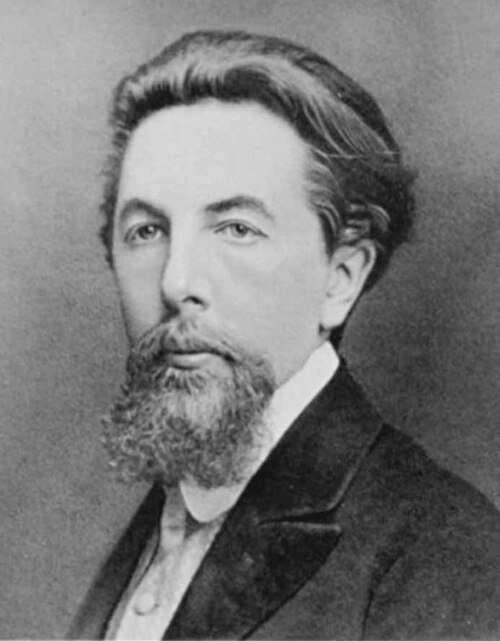
\includegraphics[width=\linewidth]{images/book3/tsvet.jpg}
\end{minipage}\hfill
\begin{minipage}[t]{0.78\linewidth}
\vspace{0pt}
The botanist Mikhail Tsvet poured an extract of green leaves onto a glass tube filled with powdered
chalk and washed it through with a solvent: the pigments separated into coloured bands, green
chlorophylls and yellow carotenoids. In 1906 he named the method \omterm{def:b2:chromatography:principle}{chromatography}, ``colour writing''.
It was largely ignored for a quarter of a century, until it was taken up again for natural products in
the 1930s. (Portrait: unknown author, public domain; Wikimedia Commons.)
\end{minipage}
\end{history}

\begin{safety}{\ghs[5mm]{GHS02}\,\ghs[5mm]{GHS05}\,\ghs[5mm]{GHS06}\,\ghs[5mm]{GHS07}\,\ghs[5mm]{GHS08}\,\ghs[5mm]{GHS09}}
Acetonitrile and methanol, the usual organic components of HPLC \omterm{def:b2:chromatography:principle}{mobile phases}, are flammable and toxic;
hexane, used in column \omterm{def:b2:chromatography:principle}{chromatography}, is flammable, a health hazard and toxic to aquatic life.
Solvent waste is collected, never poured down the sink.
% ledger: ghs:acetonitrile, ghs:methanol, ghs:hexane
\end{safety}

\section{Exercises}

\begin{exercise}[$\star$]\label{exo:b2:chromatography:1}
A compound has $t_R = \qty{5.0}{min}$ on a column whose \omterm{def:b2:chromatography:retention}{hold-up time} is \qty{1.0}{min}. Compute its
\omterm{def:b2:chromatography:retention}{retention factor} and the fraction of its time spent in the \omterm{def:b2:chromatography:principle}{mobile phase}.
\end{exercise}

\begin{exercise}[$\star$]\label{exo:b2:chromatography:2}
A peak at $t_R = \qty{6.0}{min}$ has a base width of \qty{0.30}{min}. Compute the \omterm{def:b2:chromatography:plates}{plate number}.
\end{exercise}

\begin{exercise}[$\star$]\label{exo:b2:chromatography:3}
A \qty{250}{mm} column gives $N = 10\,000$ for a compound. Compute the \omterm{def:b2:chromatography:plates}{plate height}.
\end{exercise}

\begin{exercise}[$\star$]\label{exo:b2:chromatography:4}
GC or HPLC? Ethanol in blood; a protein; caffeine in a drink; benzene in petrol; sugars in fruit juice.
\end{exercise}

\begin{exercise}[$\star\star$]\label{exo:b2:chromatography:5}
Two peaks: $t_{R1} = \qty{4.0}{min}$, $w_1 = \qty{0.40}{min}$; $t_{R2} = \qty{4.6}{min}$, $w_2 =
\qty{0.50}{min}$. Compute the \omterm{def:b2:chromatography:separation}{resolution}. Are they baseline separated?
\end{exercise}

\begin{exercise}[$\star\star$]\label{exo:b2:chromatography:6}
How many plates are needed to separate two compounds with $\alpha = 1.10$ and $k_2 = 4.0$ at
$R_s = 1.5$?
\end{exercise}

\begin{exercise}[$\star\star$]\label{exo:b2:chromatography:7}
A column has $A = \qty{5}{\micro m}$, $B = \qty{8}{\micro m.mm/s}$, $C = \qty{2}{\micro m.s/mm}$
(exercise data). Find the optimum speed and the smallest \omterm{def:b2:chromatography:plates}{plate height}.
\end{exercise}

\begin{exercise}[$\star\star$]\label{exo:b2:chromatography:8}
Predict the order of \omterm{def:b2:chromatography:principle}{elution} of benzene, phenol and toluene in reversed-phase HPLC with a
water--methanol \omterm{def:b2:chromatography:principle}{mobile phase}, and what happens when the methanol fraction is raised.
\end{exercise}

\begin{exercise}[$\star\star$]\label{exo:b2:chromatography:9}
A calibration solution of an analyte at \qty{20.0}{mg/L} with the \omterm{def:b2:chromatography:quantitative}{internal standard} at \qty{10.0}{mg/L}
gives areas 860 and 400. A sample spiked with the standard at \qty{10.0}{mg/L} gives areas 645 and 410.
Compute the \omterm{def:b2:chromatography:quantitative}{response factor} and the concentration of the analyte (exercise data).
\end{exercise}

\begin{exercise}[$\star\star\star$]\label{exo:b2:chromatography:10}
A separation gives $R_s = 1.06$. What column length, relative to the present one, gives $R_s = 1.5$, and
what does it cost in time? What other levers are there?
\end{exercise}

\begin{exercise}[$\star\star\star$]\label{exo:b2:chromatography:11}
For two Gaussian peaks of equal height and width with base width $w = 4\sigma$, compute the signal
midway between them, relative to the peak height, at $R_s = 1$ and at $R_s = 1.5$ (neglect the far
peak's contribution at each maximum).
\end{exercise}

\begin{exercise}[$\star\star\star$]\label{exo:b2:chromatography:12}
At constant $N$ and $\alpha$, compare the \omterm{def:b2:chromatography:separation}{resolution} factor $k_2/(1+k_2)$ and the relative analysis time
$1 + k_2$ for $k_2 = 2$, 5 and 10. Which range of $k$ would you choose?
\end{exercise}

\section{Problem: Caffeine in an Energy Drink}

\begin{problem}[{Weekend problem --- reversed-phase elution order, column performance from a
chromatogram, improving the separation, and quantification with an internal standard}]
\label{pb:b2:chromatography:1}
Exercise data (invented, not a real method). An energy drink is diluted tenfold (\qty{5.00}{mL} to
\qty{50.0}{mL}) and theophylline is added as \omterm{def:b2:chromatography:quantitative}{internal standard} at \qty{40.0}{mg/L} in the diluted
solution. Column: \qty{150}{mm}, \omterm{def:b2:chromatography:techniques}{reversed phase}; \omterm{def:b2:chromatography:principle}{mobile phase} water--methanol; UV detection. The
unretained matrix (sugars and salts) elutes at $t_M = \qty{1.0}{min}$; theophylline at
\qty{3.0}{min} (base width \qty{0.18}{min}); caffeine at \qty{3.4}{min} (base width \qty{0.20}{min}).
Calibration: caffeine \qty{50.0}{mg/L} and theophylline \qty{40.0}{mg/L} give areas 1500 and 1000.
Sample: areas 970 (caffeine) and 1010 (theophylline). A can holds \qty{250}{mL}.
% ledger: ghs:caffeine, ghs:methanol

\begin{center}
\begin{tikzpicture}
\begin{axis}[width=0.75\linewidth, height=4.4cm, xmin=0, xmax=5, ymin=0, ymax=1,
  xlabel={time (min)}, ylabel={absorbance (a.u.)}, label style={font=\small},
  tick label style={font=\scriptsize}, ytick=\empty]
\addplot[omDef, thick] table[x=t, y=s] {figdata/out/bachelor-2-chromatogram-c.dat};
\node[font=\scriptsize] at (axis cs:1.0,0.42) {matrix};
\node[font=\scriptsize] at (axis cs:2.62,0.86) {theophylline};
\node[font=\scriptsize] at (axis cs:3.85,0.84) {caffeine};
\end{axis}
\end{tikzpicture}
\end{center}
% figdata: bachelor-2/chromatogram.py part c

\medskip
\noindent\textbf{Part I --- \omterm{def:b2:chromatography:techniques}{Reversed phase}.}
\begin{enumerate}
  \item Describe the stationary and \omterm{def:b2:chromatography:principle}{mobile phases} of a reversed-phase column.
  \item Why do the sugars elute at the \omterm{def:b2:chromatography:retention}{hold-up time}?
  \item Caffeine is 1,3,7-trimethylxanthine, theophylline 1,3-dimethylxanthine. Explain their order of
        \omterm{def:b2:chromatography:principle}{elution}.
  \item Why is theophylline a good \omterm{def:b2:chromatography:quantitative}{internal standard} here?
  \item What would happen to both \omterm{def:b2:chromatography:retention}{retention times} if the methanol fraction were raised?
  \item What does the \omterm{def:b2:chromatography:retention}{hold-up time} measure?
\end{enumerate}

\medskip
\noindent\textbf{Part II --- Column performance.}
\begin{enumerate}[resume]
  \item Compute the \omterm{def:b2:chromatography:retention}{retention factors} of theophylline and caffeine.
  \item Compute the \omterm{def:b2:chromatography:separation}{selectivity factor}.
  \item Compute the \omterm{def:b2:chromatography:plates}{plate number} for caffeine and for theophylline.
  \item Compute the \omterm{def:b2:chromatography:plates}{plate height} for caffeine.
  \item Compute the \omterm{def:b2:chromatography:separation}{resolution} between the two peaks.
  \item Check it with the \omterm{def:b2:chromatography:separation}{resolution} equation.
  \item Are the peaks baseline separated?
\end{enumerate}

\medskip
\noindent\textbf{Part III --- Faster or better.}
\begin{enumerate}[resume]
  \item To save time, the column is shortened to \qty{75}{mm} (same packing and flow). What becomes of
        the \omterm{def:b2:chromatography:separation}{resolution}?
  \item And of the analysis time?
  \item What would a \qty{300}{mm} column give instead, and at what cost?
  \item Which lever acts on $\alpha$?
  \item Would raising $k$ help much here?
\end{enumerate}

\medskip
\noindent\textbf{Part IV --- Quantification.}
\begin{enumerate}[resume]
  \item Compute the \omterm{def:b2:chromatography:quantitative}{response factor} of caffeine relative to theophylline.
  \item Why does the injected volume not matter?
  \item Compute the concentration of caffeine in the diluted solution.
  \item Compute the concentration of caffeine in the drink.
  \item What would go wrong if a matrix compound co-eluted with theophylline?
  \item What would an external calibration require instead?
  \item State the mass of caffeine in a \qty{250}{mL} can.
\end{enumerate}
\end{problem}
